% =====================================================================================
%  ChurnAI: Calibrated, Explainable and Cost-Sensitive Customer Churn Prediction
%  IEEE conference format (IEEEtran). Compile with pdfLaTeX + BibTeX, or run
%  `uv run python scripts/compile_paper.py`. Every number, table and chart in
%  generated/ is produced by scripts/build_paper.py.
% =====================================================================================
\documentclass[conference]{IEEEtran}

\usepackage[T1]{fontenc}
\usepackage{amsmath}
\usepackage{newtxtext,newtxmath}
\usepackage[varqu,scaled=0.95]{zi4}
\renewcommand{\sfdefault}{\rmdefault}% figure text uses the body serif
\usepackage{microtype}

% Restrained palette for charts: muted blues, one brick red, one ochre accent, greys.
\usepackage{xcolor}
\definecolor{ciViolet}{HTML}{3F6A9E}
\definecolor{ciIndigo}{HTML}{3F6A9E}
\definecolor{ciCyan}{HTML}{6F9CC7}
\definecolor{ciCyanDark}{HTML}{2E5A87}
\definecolor{ciEmerald}{HTML}{1F3550}
\definecolor{ciAmber}{HTML}{B07D1A}
\definecolor{ciOrange}{HTML}{B07D1A}
\definecolor{ciCrimson}{HTML}{9E2B25}
\definecolor{ciSlate}{HTML}{7A7A7A}
\definecolor{ciInk}{HTML}{000000}
\definecolor{ciMist}{HTML}{FFFFFF}
\definecolor{ciPaper}{HTML}{FFFFFF}

\usepackage{graphicx}
\usepackage{booktabs,array,tabularx,multirow}
\usepackage{tikz}
\usetikzlibrary{arrows.meta,positioning,calc,fit,backgrounds}
\usepackage{pgfplots}
\pgfplotsset{compat=1.18}
\usepackage[caption=false,font=footnotesize]{subfig}
\usepackage{pifont}
\usepackage{cite}
\usepackage{url}
\usepackage[hidelinks]{hyperref}
\usepackage[capitalise,nameinlink]{cleveref}
\crefname{figure}{Fig.}{Figs.}\Crefname{figure}{Fig.}{Figs.}
\crefname{table}{Table}{Tables}\Crefname{table}{Table}{Tables}
\crefname{equation}{Eq.}{Eqs.}\Crefname{equation}{Eq.}{Eqs.}
\crefname{section}{Section}{Sections}\Crefname{section}{Section}{Sections}
\crefname{appendix}{Appendix}{Appendices}\Crefname{appendix}{Appendix}{Appendices}

\graphicspath{{figures/}}

% ---------------------------------------------------------------- chart & diagram styles
\pgfplotsset{
  ci base/.style={
    axis line style={black!60}, tick style={black!60},
    tick label style={font=\scriptsize, text=black},
    label style={font=\footnotesize, text=black},
    grid style={black!12}, axis x line*=bottom, axis y line*=left,
  },
  ci square/.style={width=\linewidth, height=0.95\linewidth, xmin=0, xmax=1, ymin=0, ymax=1,
    grid=major, xtick={0,0.25,0.5,0.75,1}, ytick={0,0.25,0.5,0.75,1},
    xticklabels={0,.25,.5,.75,1}, yticklabels={0,.25,.5,.75,1}},
  ci labels/.style={nodes near coords={\pgfmathprintnumber[fixed,precision=1]{\pgfplotspointmeta}\%},
    nodes near coords style={font=\scriptsize, text=black, above}},
}
\tikzset{
  ci note/.style={font=\scriptsize, fill=white, inner sep=1.5pt, draw=black!30},
  stage/.style={draw=black!70, fill=white, line width=0.5pt, minimum height=1.15cm,
    text width=2.3cm, align=center, font=\scriptsize},
  pstage/.style={draw=black!70, fill=white, line width=0.5pt, minimum height=0.74cm,
    text width=3.15cm, align=center, font=\scriptsize},
  flow/.style={-{Stealth[length=4pt]}, line width=0.55pt, color=black!75},
}

% ---------------------------------------------------------------- table helpers
\newcommand{\cmark}{\ding{51}}
\newcommand{\xmark}{\ding{55}}
\newcommand{\vbar}[1]{#1}
\newcommand{\impbar}[1]{#1}
\newcolumntype{L}{>{\raggedright\arraybackslash}X}
% Table rows are read with TeX's primitive \input: unlike LaTeX's \input it runs no file
% hooks, so a following \bottomrule still sits directly after the last \\.
\makeatletter
\newcommand{\genrows}[1]{\@@input generated/#1.tex }
\makeatother
\newcommand{\code}[1]{\texttt{#1}}
\newcommand{\para}[1]{\par\textit{#1.}\ }% IEEE-style run-in heading

% ---------------------------------------------------------------- generated content
% Auto-generated by scripts/build_paper.py -- do not edit.
\newcommand{\NCustomers}{7{,}043}
\newcommand{\NTrain}{5{,}634}
\newcommand{\NHoldout}{1{,}409}
\newcommand{\ChurnRate}{26.54\%}
\newcommand{\NChurners}{1{,}869}
\newcommand{\Champion}{ElasticNet Logistic Regression}
\newcommand{\Threshold}{0.185}
\newcommand{\HoldoutROC}{0.848}
\newcommand{\HoldoutPR}{0.651}
\newcommand{\HoldoutRecall}{86.1\%}
\newcommand{\HoldoutPrecision}{47.7\%}
\newcommand{\HoldoutFtwo}{0.742}
\newcommand{\HoldoutBrier}{0.134}
\newcommand{\HoldoutTP}{322}
\newcommand{\HoldoutFN}{52}
\newcommand{\HoldoutFP}{353}
\newcommand{\HoldoutTN}{682}
\newcommand{\HoldoutPositives}{374}
\newcommand{\CVPR}{0.655}
\newcommand{\CVPRsd}{0.018}
\newcommand{\CVROC}{0.849}
\newcommand{\CVBrier}{0.133}
\newcommand{\CVFolds}{5}
\newcommand{\CVRepeats}{2}
\newcommand{\LossChampion}{\$30{,}650}
\newcommand{\LossNone}{\$93{,}471}
\newcommand{\LossAll}{\$51{,}756}
\newcommand{\LossSavingNone}{67\%}
\newcommand{\LossSavingAll}{41\%}
\newcommand{\CostUnit}{\$50}
\newcommand{\DangerChurn}{52.9\%}
\newcommand{\LoyalChurn}{9.5\%}
\newcommand{\GenderP}{0.470}
\newcommand{\GenderChi}{0.52}
\newcommand{\ContractV}{0.410}
\newcommand{\RTenureTotal}{0.826}
\newcommand{\RMonthlyTotal}{0.651}
\newcommand{\Latency}{21}
\newcommand{\HWcpu}{Intel Core Ultra 9 285H}
\newcommand{\HWthreads}{16}
\newcommand{\HWram}{32}
\newcommand{\HWos}{Windows 11}
\newcommand{\PyVersion}{3.12.13}
\newcommand{\SklearnVersion}{1.9.1}
\newcommand{\ModelVersion}{2.0.0+20261102.elasticnet\_lr}
\newcommand{\XGBVersion}{3.4.1}
\newcommand{\LGBMVersion}{4.7.0}
\newcommand{\CatBoostVersion}{1.2.10}
\newcommand{\ShapVersion}{0.54.1}
\newcommand{\PandasVersion}{3.1.0}
\newcommand{\NumpyVersion}{2.5.4}

\newcommand{\ExampleP}{93\%}

\newcommand{\ImpMax}{0.697}


\hypersetup{
  pdftitle={ChurnAI: Calibrated, Explainable and Cost-Sensitive Customer Churn Prediction},
  pdfauthor={Krish Kamra},
  pdfkeywords={churn prediction, calibration, cost-sensitive learning, SHAP, counterfactuals}
}

\title{ChurnAI: Calibrated, Explainable and Cost-Sensitive\\ Customer Churn Prediction}
\author{\IEEEauthorblockN{Krish Kamra}
\IEEEauthorblockA{Independent Researcher\\
\url{https://github.com/KrishKamra/Customer_Churn_Prediction}}}

\begin{document}

\maketitle

\begin{abstract}
Customer churn models are usually judged on accuracy or ROC-AUC alone, and then deployed with a
default 0.5 threshold that ignores both class imbalance and the asymmetric cost of errors. We
present ChurnAI, an end-to-end, fully reproducible churn-prediction system built on the IBM Telco
dataset (\NCustomers{} customers, \ChurnRate{} churn). We first establish which behavioural
differences are statistically real: Welch and Mann--Whitney tests on continuous attributes, plus
$\chi^2$ tests with bias-corrected Cram\'er's $V$ on 16 categorical attributes. We then run a
leakage-free tournament of six learners (ElasticNet logistic regression, Balanced Random Forest,
LightGBM, XGBoost, CatBoost and a stacking ensemble). Every learner is wrapped in an identical
feature pipeline and in isotonic calibration, and each is scored with
\CVRepeats{}$\times$\CVFolds{}-fold repeated stratified cross-validation. The decision threshold
is chosen to minimise the expected cost $5\,\mathrm{FN}+1\,\mathrm{FP}$ on out-of-fold
predictions, never on the holdout. The regularised linear model wins (CV PR-AUC
\CVPR{}\,$\pm$\,\CVPRsd{}). On an untouched holdout of \NHoldout{} customers it reaches ROC-AUC
\HoldoutROC{}, PR-AUC \HoldoutPR{}, recall \HoldoutRecall{} and a Brier score of
\HoldoutBrier{}. That is \LossSavingNone{} less expected loss than doing nothing, and
\LossSavingAll{} less than a blanket retention offer. We explain predictions with SHAP and
model-based counterfactuals, audit subgroup behaviour, and ship the model behind a calibrated,
explainable dashboard with a SQL audit trail and a CI quality gate. All experiments ran on a
single laptop CPU.
\end{abstract}

\begin{IEEEkeywords}
churn prediction, probability calibration, cost-sensitive learning, SHAP, counterfactual
explanations, reproducibility
\end{IEEEkeywords}

% =====================================================================================
\section{Introduction}
\label{sec:intro}

Retaining an existing subscriber is typically far cheaper than acquiring a new one, which makes
churn prediction one of the most widely deployed applications of supervised learning in
subscription businesses \cite{neslin2006defection,verbeke2012new}. Yet the gap between a
promising notebook and a decision system that a retention team can trust is wide. Three issues
recur in practice:
\begin{enumerate}
  \item \textbf{Misaligned metrics.} With roughly one churner per three customers, accuracy
  rewards ignoring churners, and ROC-AUC hides poor precision in the region that matters
  \cite{saito2015precision,davis2006relationship}.
  \item \textbf{Uncalibrated scores and naive thresholds.} Class re-weighting and boosting
  distort probabilities \cite{niculescu2005predicting}. A fixed 0.5 threshold then ignores that a
  missed churner costs far more than a wasted retention offer \cite{elkan2001foundations}.
  \item \textbf{Opacity and leakage.} Target-derived encodings and preprocessing fitted
  before the train/validation split inflate offline metrics. Black-box scores without
  explanations are also hard to act on.
\end{enumerate}

\para{Contributions}This report documents ChurnAI, an open-source reference system
that addresses each issue:
\begin{itemize}
  \item an \textbf{inferential analysis} that separates real churn drivers from noise before
        any model is trained (\cref{sec:stats});
  \item a \textbf{leakage-free tournament} of six learners sharing one pipeline, with
        calibration inside every fold and a fingerprinted holdout (\cref{sec:method});
  \item a \textbf{cost-optimal decision rule} chosen on out-of-fold predictions, plus an
        honest analysis of threshold sensitivity (\cref{sec:results});
  \item \textbf{explanations and a subgroup audit}: global and local SHAP, counterfactual
        retention prescriptions and subgroup error rates (\cref{sec:xai,sec:fairness});
  \item a \textbf{production system}: dashboard, SQL audit log, tests and CI gate, all
        reproducible on a laptop CPU (\cref{sec:system} and the Appendix).
\end{itemize}

\Cref{tab:summary} summarises the headline results.

\begin{table}[t]
\caption{Summary of Key Results}
\label{tab:summary}
\centering
\footnotesize
\begin{tabularx}{\columnwidth}{@{}L r@{}}
\toprule
Champion (selected by CV PR-AUC) & \Champion\\
Holdout ROC-AUC / PR-AUC & \HoldoutROC{} / \HoldoutPR\\
Recall at $t=\Threshold$ & \HoldoutRecall{} (\HoldoutTP/\HoldoutPositives)\\
Brier score & \HoldoutBrier\\
Expected loss: model vs.\ no action & \LossChampion{} vs.\ \LossNone\\
Strongest categorical driver & \code{Contract} ($V=\ContractV$)\\
Churn in the first six months & \DangerChurn\\
\bottomrule
\end{tabularx}
\end{table}

% =====================================================================================
\begin{figure*}[t]
\centering
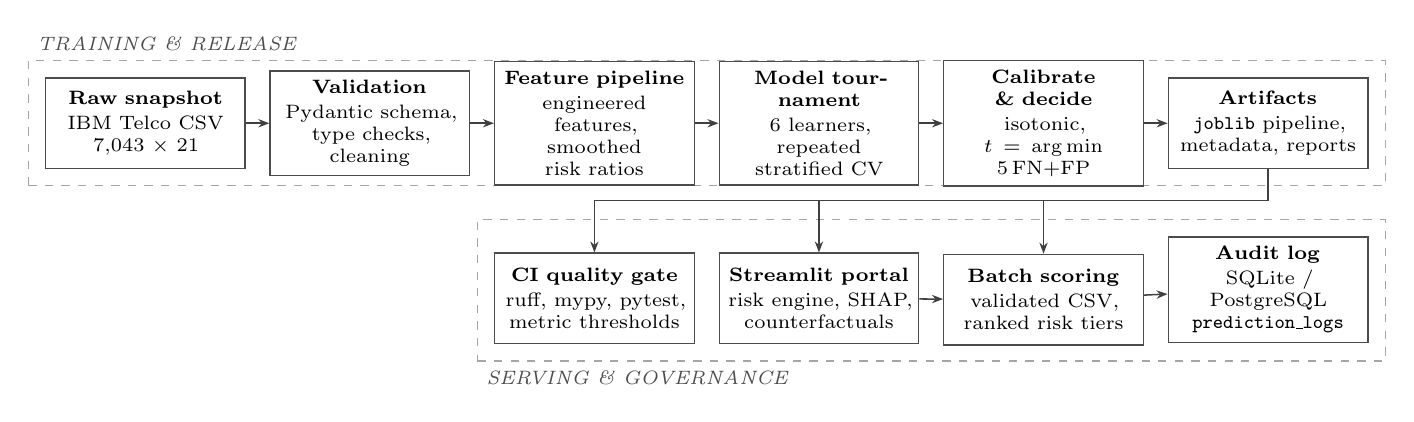
\begin{tikzpicture}[node distance=0.42cm and 0.3cm]
  \node[stage=ciCyanDark] (raw) {\textbf{Raw snapshot}\\[1pt] IBM Telco CSV\\ \NCustomers{} $\times$ 21};
  \node[stage=ciViolet, right=of raw] (val) {\textbf{Validation}\\[1pt] Pydantic schema,\\ type checks, cleaning};
  \node[stage=ciIndigo, right=of val] (feat) {\textbf{Feature pipeline}\\[1pt] engineered features,\\ smoothed risk ratios};
  \node[stage=ciEmerald, right=of feat] (tour) {\textbf{Model tournament}\\[1pt] 6 learners, repeated\\ stratified CV};
  \node[stage=ciAmber, right=of tour] (cal) {\textbf{Calibrate \& decide}\\[1pt] isotonic, $t=\arg\min$\\ $5\,$FN$+$FP};
  \node[stage=ciCrimson, right=of cal] (art) {\textbf{Artifacts}\\[1pt] \code{joblib} pipeline,\\ metadata, reports};
  \foreach \a/\b in {raw/val,val/feat,feat/tour,tour/cal,cal/art}
    \draw[flow] (\a) -- (\b);
  \node[stage=ciEmerald, below=0.85cm of feat] (ci) {\textbf{CI quality gate}\\[1pt] ruff, mypy, pytest,\\ metric thresholds};
  \node[stage=ciViolet, below=0.85cm of tour] (ui) {\textbf{Streamlit portal}\\[1pt] risk engine, SHAP,\\ counterfactuals};
  \node[stage=ciIndigo, below=0.85cm of cal] (batch) {\textbf{Batch scoring}\\[1pt] validated CSV,\\ ranked risk tiers};
  \node[stage=ciCyanDark, below=0.85cm of art] (db) {\textbf{Audit log}\\[1pt] SQLite / PostgreSQL\\ \code{prediction\_logs}};
  \draw[flow] (art.south) -- ++(0,-0.4) -| (ci.north);
  \draw[flow] (art.south) -- ++(0,-0.4) -| (ui.north);
  \draw[flow] (art.south) -- ++(0,-0.4) -| (batch.north);
  \draw[flow] (ui) -- (batch);
  \draw[flow] (batch) -- (db);
  \begin{scope}[on background layer]
    \node[fit=(raw)(art), inner sep=6pt, draw=black!35, dashed,
      label={[font=\scriptsize\itshape, text=black!70, anchor=south west]north west:TRAINING \& RELEASE}] {};
    \node[fit=(ci)(db), inner sep=6pt, draw=black!35, dashed,
      label={[font=\scriptsize\itshape, text=black!70, anchor=north west]south west:SERVING \& GOVERNANCE}] {};
  \end{scope}
\end{tikzpicture}
\caption{The ChurnAI system. One serialized pipeline is shared by training, the CI gate,
the interactive dashboard and batch scoring, so no preprocessing is ever re-implemented at
inference time.}
\label{fig:system}
\end{figure*}

% =====================================================================================
\section{Related Work}
\label{sec:related}

\para{Churn modelling}Telecom churn prediction has a long history in marketing science.
Neslin et al.~\cite{neslin2006defection} showed that modelling choices materially change the profit of
retention campaigns. Verbeke et al.~\cite{verbeke2012new} argued for profit-driven rather than
accuracy-driven evaluation, and Burez and Van den Poel~\cite{burez2009handling} studied the effect of class imbalance.
We follow this line and evaluate with PR-AUC and an explicit cost matrix.

\para{Learners}We compare an ElasticNet-regularised logistic regression
\cite{zou2005regularization}, the Balanced Random Forest \cite{chen2004using} from
imbalanced-learn \cite{lemaitre2017imbalanced}, three gradient-boosting libraries
(XGBoost \cite{chen2016xgboost}, LightGBM \cite{ke2017lightgbm}, CatBoost
\cite{prokhorenkova2018catboost}) and stacked generalisation \cite{wolpert1992stacked}. All
are implemented with scikit-learn \cite{pedregosa2011scikit}.

\para{Calibration and costs}Isotonic regression \cite{zadrozny2002transforming} and Platt
scaling correct the distorted probabilities that boosting and re-weighting produce
\cite{niculescu2005predicting}. Calibration is assessed with the Brier score
\cite{brier1950verification}. With calibrated probabilities, the cost-optimal threshold follows
directly from the cost matrix \cite{elkan2001foundations}.

\para{Explainability and accountability}SHAP \cite{lundberg2017unified} and its exact tree
variant \cite{lundberg2020local} attribute predictions to features. Counterfactual explanations
\cite{wachter2018counterfactual} answer the question a retention manager actually asks: what
would change the outcome? We document the model following model-card practice
\cite{mitchell2019model}, and we report subgroup error rates in the spirit of equality of
opportunity \cite{hardt2016equality}.

% =====================================================================================
\section{Data}
\label{sec:data}

We use the IBM Telco Customer Churn sample dataset \cite{ibmtelco}. It records
\NCustomers{} customers of a fictional telecom provider with 19 predictive attributes, a
customer identifier and a binary label: whether the customer left within the last month
(\cref{tab:dataset}). \NChurners{} customers churned (\ChurnRate{}), an imbalance of about 1:2.8.

\begin{table}[t]
\centering
\caption{Attributes of the IBM Telco dataset, grouped by type.}
\label{tab:dataset}
\footnotesize
\begin{tabularx}{\columnwidth}{@{}l L l@{}}
\toprule
\textbf{Group} & \textbf{Attributes} & \textbf{Type}\\
\midrule
Demographics & \code{gender}, \code{SeniorCitizen}, \code{Partner}, \code{Dependents} & binary\\
Services & \code{PhoneService}, \code{MultipleLines}, \code{InternetService}, \code{OnlineSecurity}, \code{OnlineBackup}, \code{DeviceProtection}, \code{TechSupport}, \code{StreamingTV}, \code{StreamingMovies} & categorical\\
Account & \code{Contract}, \code{PaperlessBilling}, \code{PaymentMethod} & categorical\\
Billing \& tenure & \code{tenure} (months), \code{MonthlyCharges}, \code{TotalCharges} & numeric\\
Label & \code{Churn} (Yes/No) & binary\\
\bottomrule
\end{tabularx}
\end{table}

\para{Cleaning}\code{TotalCharges} is stored as text, and 11 values are blank. All 11
belong to customers with $\text{tenure}=0$ who had not yet been billed, so we set them to their
true value of zero rather than imputing spend that never happened. No other values are missing.

\para{Lifecycle risk}Churn falls steeply with tenure (\cref{fig:cohort}). Customers in
their first six months churn at \DangerChurn{}, versus \LoyalChurn{} after four years. This
\emph{danger zone} is the single clearest operational finding in the data.

\begin{figure}[t]
\centering
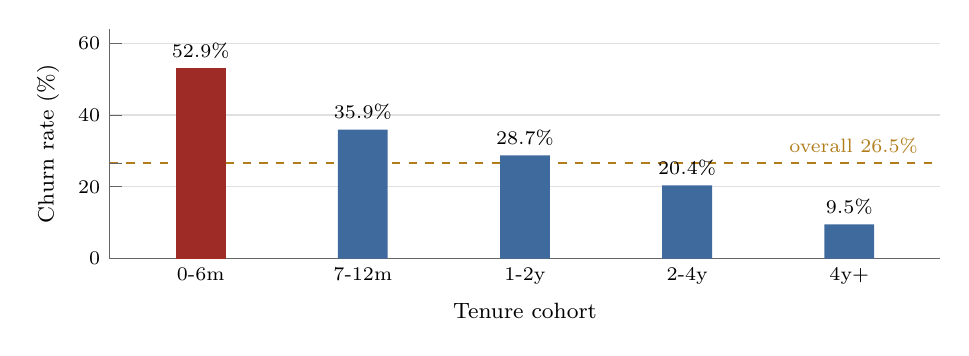
\begin{tikzpicture}
\begin{axis}[ci base, width=\columnwidth, height=4.5cm, symbolic x coords={0-6m,7-12m,1-2y,2-4y,4y+},
  xtick={0-6m,7-12m,1-2y,2-4y,4y+}, ymin=0, ymax=64, ylabel={Churn rate (\%)}, xlabel={Tenure cohort},
  enlarge x limits=0.14, ymajorgrids,
  extra y ticks={26.54}, extra y tick labels={},
  extra y tick style={grid=major, major grid style={ciAmber, dashed, thick}}]
\addplot[ybar, bar width=18pt, bar shift=0pt, fill=ciCrimson, draw=none, ci labels]
  coordinates {(0-6m,52.94)};
\addplot[ybar, bar width=18pt, bar shift=0pt, fill=ciViolet, draw=none, ci labels]
  coordinates {(7-12m,35.89) (1-2y,28.71) (2-4y,20.39) (4y+,9.51)};
\node[font=\scriptsize\sffamily, text=ciAmber, anchor=south east]
  at (rel axis cs:0.985,0.4146) {overall 26.5\%};
\end{axis}
\end{tikzpicture}

\caption{Churn rate by tenure cohort. The 0--6 month danger zone (red) churns at more than
twice the overall rate (dashed line).}
\label{fig:cohort}
\end{figure}

\para{Redundancy}\code{TotalCharges} is close to tenure times monthly charges:
its correlation with tenure is $r=\RTenureTotal$ (\cref{fig:corr}). Rather than drop it, we add a
\emph{charge-velocity ratio} that keeps only the residual information, such as plan changes and
discounts (\cref{sec:method}).

\begin{figure}[t]
\centering
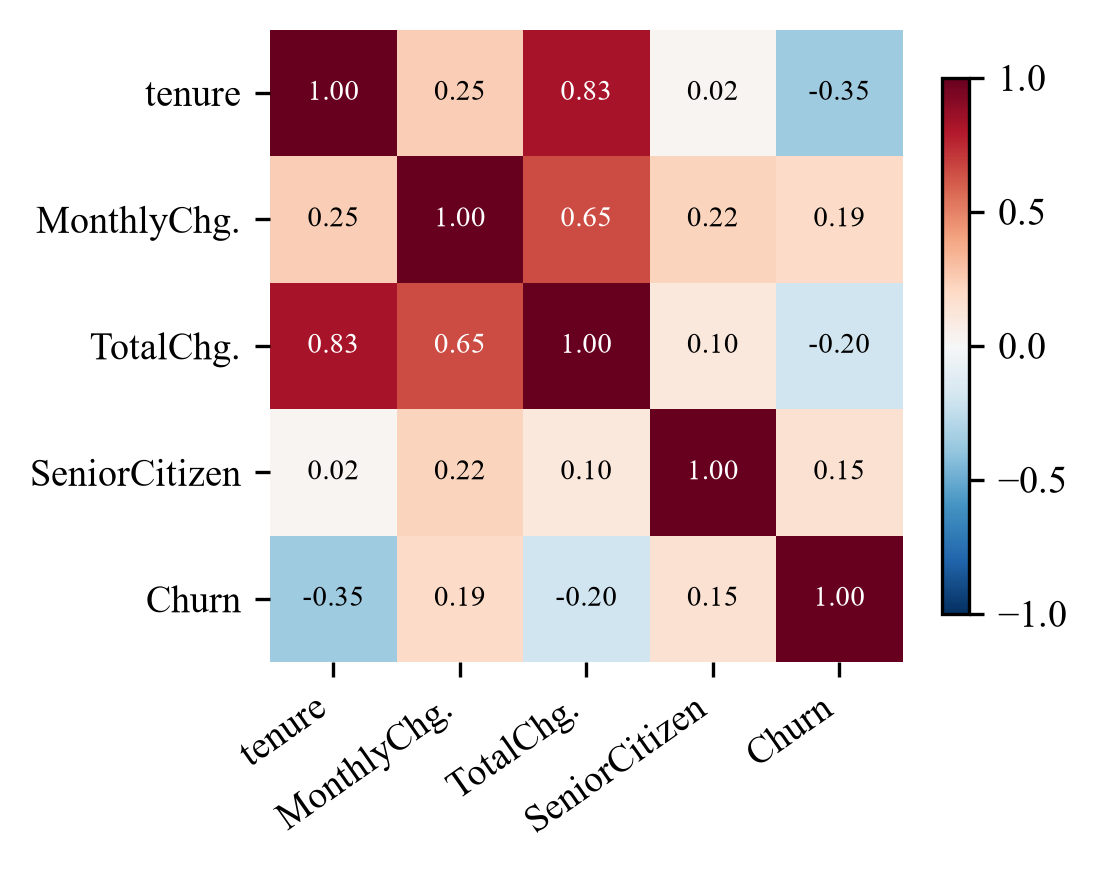
\includegraphics[width=0.86\columnwidth]{correlation_light.png}
\caption{Pearson correlations among the numeric attributes and the label.}
\label{fig:corr}
\end{figure}

% =====================================================================================
\section{Inferential Analysis}
\label{sec:stats}

Before training models, we test which differences between churners and retained customers are
statistically real, using $\alpha=0.05$.

\para{Continuous attributes}Normality (Shapiro--Wilk) and equal variances (Levene) are
both rejected for every attribute. We therefore pair Welch's $t$-test \cite{welch1947generalization}
with the distribution-free Mann--Whitney $U$ test \cite{mann1947test}, and report the
rank-biserial correlation as an effect size (\cref{tab:continuous}). Churners have markedly
shorter tenure and lower lifetime spend but \emph{higher} monthly charges: they are new
customers on expensive plans. The two tests agree on every variable.

\begin{table*}[t]
\centering
\caption{Continuous attributes, churned vs.\ retained customers. $r_{rb}$ is the rank-biserial
correlation; positive values mean churners rank lower.}
\label{tab:continuous}
\small
\begin{tabular}{@{}l rr r rr r@{}}
\toprule
& \multicolumn{2}{c}{\textbf{Mean}} & & \multicolumn{2}{c}{\textbf{$p$-value}} & \\
\cmidrule(lr){2-3}\cmidrule(lr){5-6}
\textbf{Attribute} & Churned & Retained & Welch $t$ & Welch & Mann--Whitney & $r_{rb}$\\
\midrule
\genrows{tab_continuous}
\bottomrule
\end{tabular}
\end{table*}

\para{Categorical attributes}For each of the 16 categorical attributes (the 15 string
attributes plus \code{SeniorCitizen}) we test independence from churn with a $\chi^2$ test. We
measure association strength with Cram\'er's $V$ \cite{cramer1946mathematical}, using the
bias-corrected estimator of Bergsma~\cite{bergsma2013bias}:
\begin{align}
  \tilde V &= \sqrt{\frac{\tilde\varphi^2}{\min(\tilde k-1,\tilde r-1)}},\label{eq:cramer}\\
  \tilde\varphi^2 &= \max\!\Big(0,\frac{\chi^2}{n}-\frac{(k-1)(r-1)}{n-1}\Big),\nonumber
\end{align}
with $\tilde k=k-(k-1)^2/(n-1)$, and $\tilde r$ defined analogously. \Cref{tab:chisq} ranks the
attributes. \code{Contract} is the strongest driver ($V=\ContractV$), followed by the absence
of security and support add-ons, fiber internet and electronic-check payment. \code{gender}
($\chi^2=\GenderChi$, $p=\GenderP$) and \code{PhoneService} are independent of churn. This
gender result anchors the subgroup audit in \cref{sec:fairness}.

\begin{table*}[t]
\centering
\caption{$\chi^2$ test of independence and bias-corrected Cram\'er's $V$ for all 16 categorical
attributes, ranked by effect size. The last column shows the attribute level with the highest
churn rate.}
\label{tab:chisq}
\small
\begin{tabular}{@{}r l r r r l c l@{}}
\toprule
\textbf{\#} & \textbf{Attribute} & $\chi^2$ & dof & $p$-value & \textbf{Cram\'er's $V$} & Sig. & \textbf{Highest-risk level}\\
\midrule
\genrows{tab_chisq}
\bottomrule
\end{tabular}
\end{table*}

% =====================================================================================
\section{Method}
\label{sec:method}

\subsection{Feature pipeline}
Every learner receives the same scikit-learn pipeline. Its first stage is a stateless
\code{FeatureEngineer} that never sees the label, so it is safe to apply anywhere. It adds
seven numeric features and one categorical one: $\log(1+x)$ transforms of both charge
variables, the number of add-on services, fiber/month-to-month and automatic-payment flags,
average monthly spend, a tenure cohort, and the charge-velocity ratio
\begin{equation}
  v = \frac{\text{TotalCharges}}{\text{tenure}\cdot\text{MonthlyCharges}+\epsilon},\qquad v\in[0,5].
  \label{eq:velocity}
\end{equation}
A target-aware \code{RiskRatioEncoder} then encodes three high-churn interactions
(Internet$\times$Contract, Contract$\times$Payment, Cohort$\times$Contract) as smoothed risk ratios
\begin{equation}
  \rho(g)=\frac{1}{\pi}\cdot\frac{n_g\,\bar y_g+m\,\pi}{n_g+m},\qquad m=20,
  \label{eq:riskratio}
\end{equation}
where $\pi$ is the training-fold churn rate and $\bar y_g$ the churn rate of group $g$. Unseen
groups encode to $\rho=1$. Finally, numeric columns are median-imputed and standardised, and
categorical columns are one-hot encoded with unknown levels ignored. Because the encoder and
every learned transform sit \emph{inside} the pipeline, they are re-fit on each training fold,
which removes the most common source of leakage.

\subsection{Learners}
\Cref{tab:hyper} lists the six contenders and their regularised defaults. Imbalance is handled
by class weighting (\code{balanced}, \code{scale\_pos\_weight}) or balanced bootstrap sampling,
never by synthetic oversampling.

\begin{table}[t]
\centering
\caption{Tournament contenders and their main settings.}
\label{tab:hyper}
\footnotesize
\begin{tabularx}{\columnwidth}{@{}l L@{}}
\toprule
\textbf{Model} & \textbf{Key settings}\\
\midrule
ElasticNet LR & \code{saga}, $C=0.5$, $\ell_1$ ratio $0.5$, balanced class weights\\
Balanced RF & 400 trees, min leaf 3, $\sqrt{p}$ features, per-tree undersampling\\
LightGBM & 500 trees, lr $0.03$, 15 leaves, row/col subsample $0.8$, $\lambda=2$\\
XGBoost & 400 trees, lr $0.03$, depth 4, \code{hist}, subsample $0.8$, $\lambda=2$\\
CatBoost & 600 iterations, lr $0.04$, depth 5, $\ell_2=5$, balanced weights\\
Stacking & CatBoost + XGBoost + ElasticNet LR $\rightarrow$ logistic meta-learner (5-fold)\\
\bottomrule
\end{tabularx}
\end{table}

\subsection{Evaluation protocol}
\Cref{fig:protocol} summarises the protocol. A stratified 80/20 split with a fixed seed reserves
\NHoldout{} customers as a holdout. We store the SHA-256 fingerprint of the holdout customer IDs,
and the CI gate refuses to evaluate if it changes. On the \NTrain{} training customers, each
contender, wrapped in isotonic \code{CalibratedClassifierCV}, is scored with repeated stratified
\CVFolds{}-fold CV ($\times$\CVRepeats{} repeats).

\begin{figure}[t]
\centering
\begin{tikzpicture}[node distance=0.32cm]
  \node[pstage=ciCyanDark, text width=6.6cm] (data) {\textbf{IBM Telco} \quad \NCustomers{} customers};
  \node[pstage=ciViolet, below=0.5cm of data.south west, anchor=north west] (train) {\textbf{Training split}\\ \NTrain{} customers};
  \node[pstage=ciCrimson, below=0.5cm of data.south east, anchor=north east] (hold) {\textbf{Holdout split}\\ \NHoldout{} \textbullet\ SHA-256 fingerprint};
  \node[pstage=ciIndigo, below=of train] (cv) {Repeated stratified\\ \CVFolds{}-fold CV $\times$ \CVRepeats{}};
  \node[pstage=ciIndigo, below=of cv] (fold) {per fold: fit pipeline\\ + isotonic calibration};
  \node[pstage=ciEmerald, below=of fold] (sel) {champion $=\arg\max$ PR-AUC};
  \node[pstage=ciAmber, below=of sel] (thr) {$t=\arg\min_t\,5\mathrm{FN}+\mathrm{FP}$\\ on out-of-fold scores};
  \node[pstage=ciEmerald, below=of thr] (fit) {refit champion\\ on full training split};
  \node[pstage=ciCrimson, below=of fit, xshift=0cm] (eval) {\textbf{one-time evaluation}\\ \& CI quality gate};
  \draw[flow] (data.south) ++(-1.6,0) -- (train.north);
  \draw[flow] (data.south) ++(1.6,0) -- (hold.north);
  \foreach \a/\b in {train/cv,cv/fold,fold/sel,sel/thr,thr/fit,fit/eval} \draw[flow] (\a) -- (\b);
  \draw[flow, dashed] (hold.south) |- (eval.east);
  \node[font=\tiny\itshape, align=left, anchor=west] at ([xshift=0.3cm]hold.south |- thr.east)
    {never used for\\ selection, tuning,\\ calibration or\\ threshold choice};
\end{tikzpicture}
\caption{Evaluation protocol. The holdout is touched exactly once.}
\label{fig:protocol}
\end{figure}

\para{Metrics}The primary metric is PR-AUC (average precision), which is more informative
than ROC-AUC under imbalance \cite{saito2015precision}. Secondary metrics are ROC-AUC, the
Brier score $B=\frac1n\sum_i(p_i-y_i)^2$ \cite{brier1950verification}, recall, precision,
$F_2$, and the business cost
\begin{equation}
  \mathcal{C}(t)=c_{\mathrm{FN}}\cdot\mathrm{FN}(t)+c_{\mathrm{FP}}\cdot\mathrm{FP}(t),\qquad
  c_{\mathrm{FN}}=5,\;c_{\mathrm{FP}}=1,
  \label{eq:cost}
\end{equation}
where one cost unit (one wasted retention offer) is valued at \CostUnit{}. This is an
illustrative assumption, and it is configurable.

\para{Decision threshold}For perfectly calibrated probabilities, the Bayes-optimal rule
intervenes when $p\geq t^\ast=c_{\mathrm{FP}}/(c_{\mathrm{FP}}+c_{\mathrm{FN}})=1/6$
\cite{elkan2001foundations}. We correct for residual miscalibration by minimising \cref{eq:cost}
over a threshold grid on the out-of-fold probabilities. We take the median across repeats,
which gives $t=\Threshold$ for the champion. This is close to $1/6$, which itself suggests the
probabilities are well calibrated.

\para{Tuning}After selection, a 30-iteration randomised search over the champion's
hyper-parameters (here, $C$ and the $\ell_1$ ratio) is re-scored with the same CV protocol. Its
result is adopted only if it improves mean CV PR-AUC. In our run it did not, so the regularised
defaults were kept.

% =====================================================================================
\section{Results}
\label{sec:results}

\subsection{Cross-validated tournament}
\Cref{tab:cv} and \cref{fig:models} report the tournament. The ElasticNet logistic regression
achieves the highest mean PR-AUC, but the top three contenders are separated by less than one
standard deviation. On a dataset whose non-leaky ceiling is around ROC-AUC 0.85, extra model
capacity buys almost nothing. The stacking ensemble ties the linear model on ROC-AUC and Brier
score, while taking about 24$\times$ longer to fit.

\begin{table*}[t]
\centering
\caption{Repeated stratified cross-validation on the training split (mean $\pm$ SD over
\CVRepeats{}$\times$\CVFolds{} folds; each fold re-fits the pipeline and calibration). Cost per customer
uses each model's out-of-fold cost-optimal threshold. $^\star$\,champion.}
\label{tab:cv}
\small
\begin{tabular}{@{}l c c c c r@{}}
\toprule
\textbf{Model} & \textbf{PR-AUC} $\uparrow$ & \textbf{ROC-AUC} $\uparrow$ & \textbf{Brier} $\downarrow$ & \textbf{Cost / customer} $\downarrow$ & \textbf{Fit (s)}\\
\midrule
\genrows{tab_cv}
\bottomrule
\end{tabular}
\end{table*}

\begin{figure}[t]
\centering
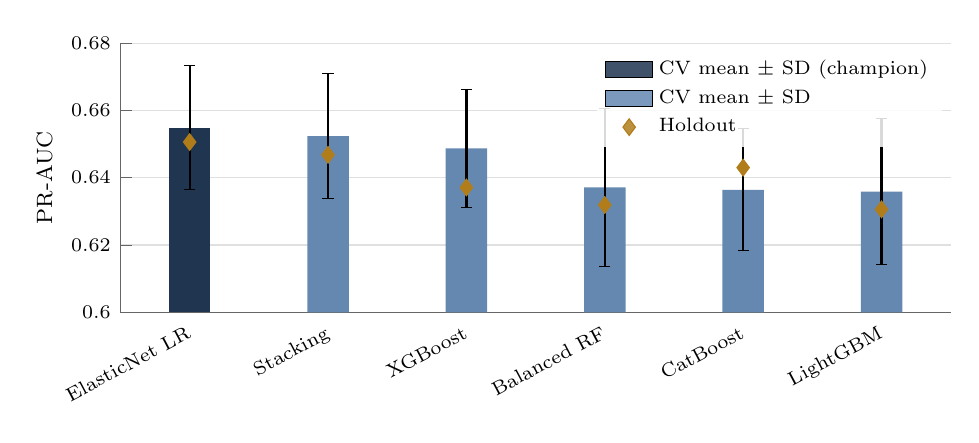
\begin{tikzpicture}
\begin{axis}[ci base, width=\columnwidth, height=5cm, symbolic x coords={ElasticNet LR,Stacking,XGBoost,Balanced RF,CatBoost,LightGBM},
  xtick={ElasticNet LR,Stacking,XGBoost,Balanced RF,CatBoost,LightGBM}, x tick label style={rotate=28, anchor=north east, font=\scriptsize\sffamily},
  ymin=0.60, ymax=0.68, ylabel={PR-AUC}, enlarge x limits=0.1, ymajorgrids,
  y tick label style={/pgf/number format/fixed, /pgf/number format/precision=2},
  legend style={at={(0.99,0.98)}, anchor=north east, font=\scriptsize\sffamily,
  draw=none, fill=white, fill opacity=0.85, text opacity=1}, legend cell align=left]
\addplot[ybar, bar width=15pt, bar shift=0pt, fill=ciEmerald, draw=none, area legend, error bars/.cd, y dir=both, y explicit, error bar style={ciInk, thick}]
  coordinates {(ElasticNet LR,0.6549) +- (0,0.0184)};
\addlegendentry{CV mean $\pm$ SD (champion)}
\addplot[ybar, bar width=15pt, bar shift=0pt, fill=ciViolet!80, draw=none, area legend, error bars/.cd, y dir=both, y explicit, error bar style={ciInk, thick}]
  coordinates {(Stacking,0.6524) +- (0,0.0185) (XGBoost,0.6487) +- (0,0.0176) (Balanced RF,0.6371) +- (0,0.0236) (CatBoost,0.6364) +- (0,0.0181) (LightGBM,0.6359) +- (0,0.0217)};
\addlegendentry{CV mean $\pm$ SD}
\addplot[only marks, mark=diamond*, mark size=3pt, color=ciAmber]
  coordinates {(ElasticNet LR,0.6506) (Stacking,0.6468) (XGBoost,0.6371) (Balanced RF,0.6319) (CatBoost,0.6430) (LightGBM,0.6306)};
\addlegendentry{Holdout}
\end{axis}
\end{tikzpicture}

\caption{Cross-validated PR-AUC ($\pm$1 SD) and holdout PR-AUC (diamonds). The differences
among the top contenders lie within fold-to-fold noise.}
\label{fig:models}
\end{figure}

\subsection{Holdout performance}
\Cref{tab:holdout} scores every contender once on the untouched holdout, each at its own
out-of-fold threshold. The champion attains ROC-AUC \HoldoutROC{}, PR-AUC \HoldoutPR{} and the
best calibration (Brier \HoldoutBrier{}). At $t=\Threshold$ it identifies \HoldoutTP{} of the
\HoldoutPositives{} churners (recall \HoldoutRecall{}) at a precision of \HoldoutPrecision{}.
XGBoost records a marginally lower expected loss on this particular split. The gap (about 3\%)
is well within the variation between CV folds, and we keep the pre-registered selection rule
rather than pick a winner on the holdout. \Cref{fig:curves} shows the champion's ROC,
precision--recall and reliability curves.

\begin{table*}[t]
\centering
\caption{Holdout evaluation (\NHoldout{} customers). Each model uses its own cost-optimal
threshold $t$ from out-of-fold predictions. Latency is the median single-row
\code{predict\_proba} time of the full pipeline on a laptop CPU. Rows are sorted by expected
loss. $^\star$\,champion.}
\label{tab:holdout}
\small
\begin{tabular}{@{}l c c c c c c c r r@{}}
\toprule
\textbf{Model} & $t$ & \textbf{ROC-AUC} & \textbf{PR-AUC} & \textbf{Recall} & \textbf{Precision} & $\boldsymbol{F_2}$ & \textbf{Brier} & \textbf{ms} & \textbf{Loss (\$)}\\
\midrule
\genrows{tab_holdout}
\bottomrule
\end{tabular}
\end{table*}

\begin{figure*}[t]
\centering
\subfloat[ROC curve]{\begin{minipage}{0.31\textwidth}\centering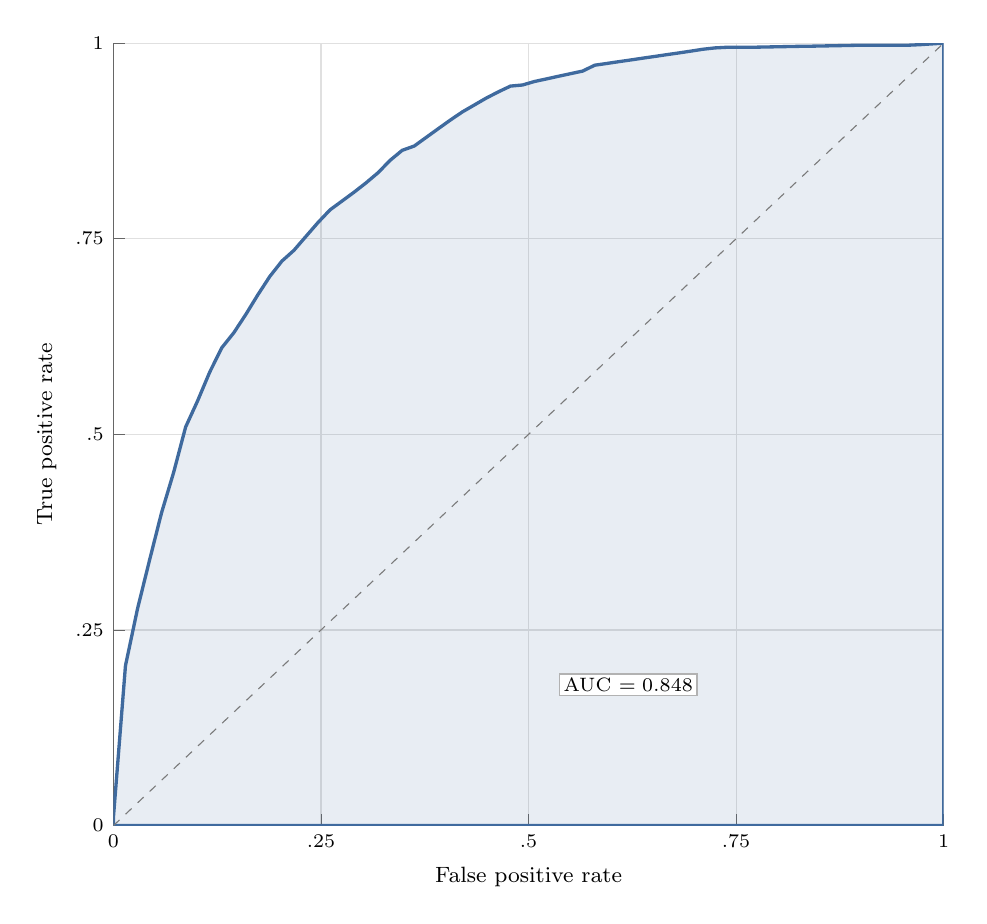
\begin{tikzpicture}
\begin{axis}[ci base, ci square, xlabel={False positive rate}, ylabel={True positive rate}]
\addplot[draw=ciViolet, very thick, fill=ciViolet, fill opacity=0.12] coordinates {(0.0,0.0107) (0.014492753623188406,0.2044) (0.028985507246376812,0.2770) (0.043478260869565216,0.3392) (0.057971014492753624,0.3999) (0.07246376811594203,0.4512) (0.08695652173913043,0.5094) (0.10144927536231885,0.5430) (0.11594202898550725,0.5795) (0.13043478260869565,0.6106) (0.14492753623188406,0.6298) (0.15942028985507248,0.6532) (0.17391304347826086,0.6783) (0.18840579710144928,0.7019) (0.2028985507246377,0.7214) (0.21739130434782608,0.7352) (0.2318840579710145,0.7530) (0.2463768115942029,0.7707) (0.2608695652173913,0.7869) (0.2753623188405797,0.7982) (0.2898550724637681,0.8095) (0.30434782608695654,0.8215) (0.31884057971014496,0.8345) (0.3333333333333333,0.8503) (0.34782608695652173,0.8630) (0.36231884057971014,0.8685) (0.37681159420289856,0.8796) (0.391304347826087,0.8907) (0.4057971014492754,0.9017) (0.42028985507246375,0.9121) (0.43478260869565216,0.9210) (0.4492753623188406,0.9299) (0.463768115942029,0.9378) (0.4782608695652174,0.9451) (0.4927536231884058,0.9465) (0.5072463768115942,0.9510) (0.5217391304347826,0.9543) (0.5362318840579711,0.9577) (0.5507246376811594,0.9610) (0.5652173913043478,0.9643) (0.5797101449275363,0.9718) (0.5942028985507246,0.9740) (0.6086956521739131,0.9763) (0.6231884057971014,0.9785) (0.6376811594202899,0.9808) (0.6521739130434783,0.9830) (0.6666666666666666,0.9853) (0.6811594202898551,0.9875) (0.6956521739130435,0.9898) (0.7101449275362319,0.9922) (0.7246376811594203,0.9939) (0.7391304347826088,0.9947) (0.7536231884057971,0.9947) (0.7681159420289855,0.9947) (0.782608695652174,0.9950) (0.7971014492753623,0.9953) (0.8115942028985508,0.9956) (0.8260869565217391,0.9959) (0.8405797101449275,0.9961) (0.855072463768116,0.9964) (0.8695652173913043,0.9967) (0.8840579710144928,0.9970) (0.8985507246376812,0.9973) (0.9130434782608696,0.9973) (0.927536231884058,0.9973) (0.9420289855072463,0.9973) (0.9565217391304348,0.9973) (0.9710144927536232,0.9980) (0.9855072463768116,0.9990) (1.0,1.0000)} \closedcycle;
\addplot[ciSlate, dashed] coordinates {(0,0) (1,1)};
\node[ci note] at (rel axis cs:0.62,0.18) {AUC $= 0.848$};
\end{axis}
\end{tikzpicture}
\end{minipage}}\hfill
\subfloat[Precision--recall curve]{\begin{minipage}{0.31\textwidth}\centering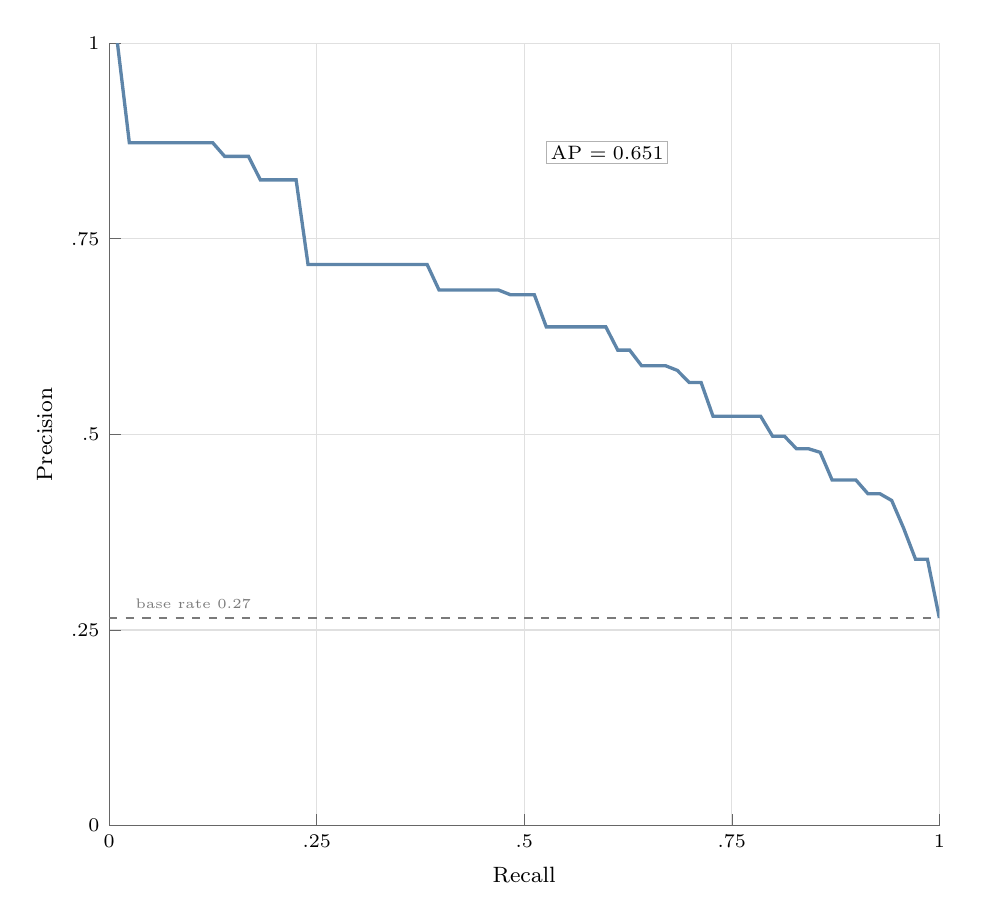
\begin{tikzpicture}
\begin{axis}[ci base, ci square, xlabel={Recall}, ylabel={Precision}]
\addplot[draw=ciCyan!85!black, very thick] coordinates {(0.01,1.0000) (0.02434782608695652,0.8727) (0.03869565217391304,0.8727) (0.05304347826086957,0.8727) (0.06739130434782609,0.8727) (0.0817391304347826,0.8727) (0.09608695652173913,0.8727) (0.11043478260869564,0.8727) (0.12478260869565216,0.8727) (0.1391304347826087,0.8553) (0.15347826086956523,0.8553) (0.16782608695652174,0.8553) (0.18217391304347827,0.8252) (0.19652173913043477,0.8252) (0.2108695652173913,0.8252) (0.2252173913043478,0.8252) (0.23956521739130435,0.7171) (0.2539130434782609,0.7171) (0.2682608695652174,0.7171) (0.2826086956521739,0.7171) (0.29695652173913045,0.7171) (0.31130434782608696,0.7171) (0.32565217391304346,0.7171) (0.33999999999999997,0.7171) (0.35434782608695653,0.7171) (0.36869565217391304,0.7171) (0.38304347826086954,0.7171) (0.3973913043478261,0.6844) (0.4117391304347826,0.6844) (0.4260869565217391,0.6844) (0.4404347826086956,0.6844) (0.4547826086956522,0.6844) (0.4691304347826087,0.6844) (0.4834782608695652,0.6784) (0.49782608695652175,0.6784) (0.5121739130434783,0.6784) (0.5265217391304348,0.6374) (0.5408695652173913,0.6374) (0.5552173913043478,0.6374) (0.5695652173913043,0.6374) (0.5839130434782609,0.6374) (0.5982608695652174,0.6374) (0.6126086956521739,0.6077) (0.6269565217391304,0.6077) (0.6413043478260869,0.5878) (0.6556521739130434,0.5878) (0.6699999999999999,0.5878) (0.6843478260869565,0.5818) (0.698695652173913,0.5663) (0.7130434782608696,0.5663) (0.7273913043478261,0.5231) (0.7417391304347826,0.5231) (0.7560869565217391,0.5231) (0.7704347826086956,0.5231) (0.7847826086956522,0.5231) (0.7991304347826087,0.4976) (0.8134782608695652,0.4976) (0.8278260869565217,0.4817) (0.8421739130434782,0.4817) (0.8565217391304347,0.4770) (0.8708695652173912,0.4416) (0.8852173913043478,0.4416) (0.8995652173913044,0.4416) (0.9139130434782609,0.4242) (0.9282608695652174,0.4242) (0.9426086956521739,0.4155) (0.9569565217391304,0.3801) (0.9713043478260869,0.3404) (0.9856521739130435,0.3404) (1.0,0.2654)};
\addplot[ciSlate, dashed] coordinates {(0,0.2654) (1,0.2654)};
\node[ci note] at (rel axis cs:0.6,0.86) {AP $= 0.651$};
\node[font=\tiny\sffamily, text=ciSlate, anchor=south west] at (axis cs:0.02,0.2654) {base rate 0.27};
\end{axis}
\end{tikzpicture}
\end{minipage}}\hfill
\subfloat[Reliability diagram (deciles)]{\begin{minipage}{0.31\textwidth}\centering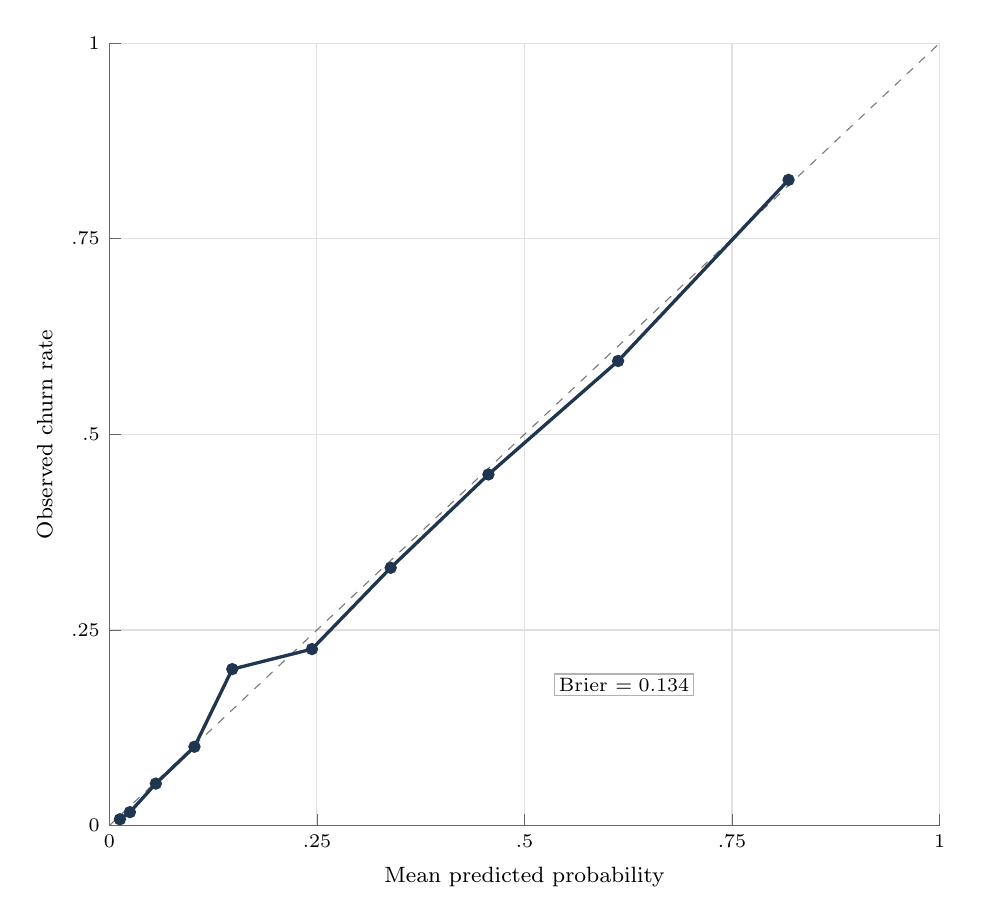
\begin{tikzpicture}
\begin{axis}[ci base, ci square, xlabel={Mean predicted probability}, ylabel={Observed churn rate}]
\addplot[ciSlate, dashed] coordinates {(0,0) (1,1)};
\addplot[ciEmerald, very thick, mark=*, mark size=1.6pt] coordinates {(0.01268246135052928,0.0081) (0.024746572316490287,0.0172) (0.05594630872483211,0.0537) (0.10249370012398486,0.1008) (0.1480226856348764,0.2000) (0.2440246723026318,0.2256) (0.3388179913656284,0.3295) (0.4565830041707477,0.4488) (0.6127352576908229,0.5938) (0.8180755644440872,0.8252)};
\node[ci note] at (rel axis cs:0.62,0.18) {Brier $= 0.134$};
\end{axis}
\end{tikzpicture}
\end{minipage}}
\caption{Holdout diagnostics for the champion. Ranking quality (a, b) is strong, and the
isotonic-calibrated probabilities track observed churn rates closely (c). That is what makes the
probabilities usable for cost-based decisions and for revenue-at-risk estimates.}
\label{fig:curves}
\end{figure*}

\subsection{Business cost and threshold sensitivity}
The cost-optimal threshold transforms the model's value (\cref{fig:cost}). On the holdout,
doing nothing costs \LossNone{} and a blanket offer to every customer costs \LossAll{}. The
champion at $t=\Threshold$ costs \LossChampion{}, which is \LossSavingNone{} and
\LossSavingAll{} lower respectively. The naive 0.5 threshold would forgo much of this gain.
\Cref{tab:threshold} shows that the loss curve is flat between $t\approx0.10$ and $0.20$. The
exact threshold matters far less than moving away from 0.5. Within that flat region, the choice
trades recall for retention-team workload.

\begin{figure}[t]
\centering
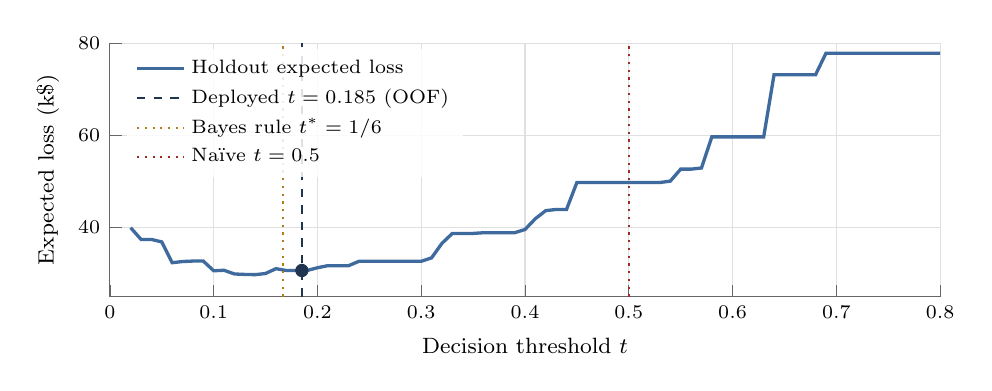
\begin{tikzpicture}
\begin{axis}[ci base, width=\columnwidth, height=4.8cm, xmin=0, xmax=0.8, ymin=25.0, ymax=80.0,
  xlabel={Decision threshold $t$}, ylabel={Expected loss (k\$)}, ymajorgrids, xmajorgrids,
  legend style={at={(0.02,0.98)}, anchor=north west, font=\scriptsize\sffamily, draw=none,
  fill=white, fill opacity=0.85, text opacity=1}, legend cell align=left]
\addplot[ciViolet, very thick] coordinates {(0.02,39.950) (0.03,37.400) (0.04,37.400) (0.05,36.850) (0.06,32.350) (0.07,32.600) (0.08,32.700) (0.09,32.700) (0.1,30.600) (0.11,30.700) (0.12,29.900) (0.13,29.800) (0.14,29.750) (0.15,30.000) (0.16,31.050) (0.17,30.650) (0.18,30.650) (0.19,30.650) (0.2,31.250) (0.21,31.700) (0.22,31.700) (0.23,31.700) (0.24,32.650) (0.25,32.650) (0.26,32.650) (0.27,32.650) (0.28,32.650) (0.29,32.650) (0.3,32.650) (0.31,33.400) (0.32,36.550) (0.33,38.700) (0.34,38.700) (0.35,38.700) (0.36,38.850) (0.37,38.850) (0.38,38.850) (0.39,38.850) (0.4,39.550) (0.41,41.900) (0.42,43.650) (0.43,43.900) (0.44,43.900) (0.45,49.750) (0.46,49.750) (0.47,49.750) (0.48,49.750) (0.49,49.750) (0.5,49.750) (0.51,49.750) (0.52,49.750) (0.53,49.750) (0.54,50.050) (0.55,52.650) (0.56,52.650) (0.57,52.900) (0.58,59.650) (0.59,59.650) (0.6,59.650) (0.61,59.650) (0.62,59.650) (0.63,59.650) (0.64,73.150) (0.65,73.150) (0.66,73.150) (0.67,73.150) (0.68,73.150) (0.69,77.800) (0.7,77.800) (0.71,77.800) (0.72,77.800) (0.73,77.800) (0.74,77.800) (0.75,77.800) (0.76,77.800) (0.77,77.800) (0.78,77.800) (0.79,77.800) (0.8,77.800)};
\addlegendentry{Holdout expected loss}
\addlegendimage{ciEmerald, thick, dashed}\addlegendentry{Deployed $t=0.185$ (OOF)}
\addlegendimage{ciAmber, thick, dotted}\addlegendentry{Bayes rule $t^\ast=1/6$}
\addlegendimage{ciCrimson, thick, dotted}\addlegendentry{Na\"ive $t=0.5$}
\draw[ciEmerald, thick, dashed] (axis cs:0.1850,25.0) -- (axis cs:0.1850,80.0);
\draw[ciAmber, thick, dotted] (axis cs:0.1667,25.0) -- (axis cs:0.1667,80.0);
\draw[ciCrimson, thick, dotted] (axis cs:0.5000,25.0) -- (axis cs:0.5000,80.0);
\addplot[only marks, mark=*, mark size=2.2pt, ciEmerald] coordinates {(0.1850,30.650)};
\end{axis}
\end{tikzpicture}

\caption{Expected holdout loss as a function of the decision threshold. The deployed threshold
was chosen on out-of-fold data and lies in the flat optimum, next to the Bayes rule $1/6$.}
\label{fig:cost}
\end{figure}

\begin{table}[t]
\centering
\caption{Threshold sensitivity of the champion on the holdout. $^\dagger$\,deployed threshold
(chosen out-of-fold).}
\label{tab:threshold}
\footnotesize
\setlength{\tabcolsep}{4.5pt}
\begin{tabular}{@{}l c c r r r r@{}}
\toprule
$t$ & \textbf{Recall} & \textbf{Prec.} & TP & FP & FN & \textbf{Loss (\$)}\\
\midrule
\genrows{tab_threshold}
\bottomrule
\end{tabular}
\end{table}

% =====================================================================================
\section{Explainability}
\label{sec:xai}

\para{Global}For linear and tree champions, SHAP values are exact (LinearSHAP or
TreeSHAP \cite{lundberg2017unified,lundberg2020local}). They are computed in log-odds space on the
inner, pre-calibration pipeline. Isotonic calibration is monotone, so signs and rankings carry
over to the deployed probability. We sum the SHAP values of one-hot columns back to their source
attribute. \Cref{fig:shap,tab:importance} show that lifecycle features dominate: the
cohort$\times$contract risk ratio, lifetime spend, average monthly spend and the tenure cohort.
Internet service, contract type and missing security add-ons follow. These are the same drivers the
inferential analysis identified independently in \cref{sec:stats}.

\begin{figure}[t]
\centering
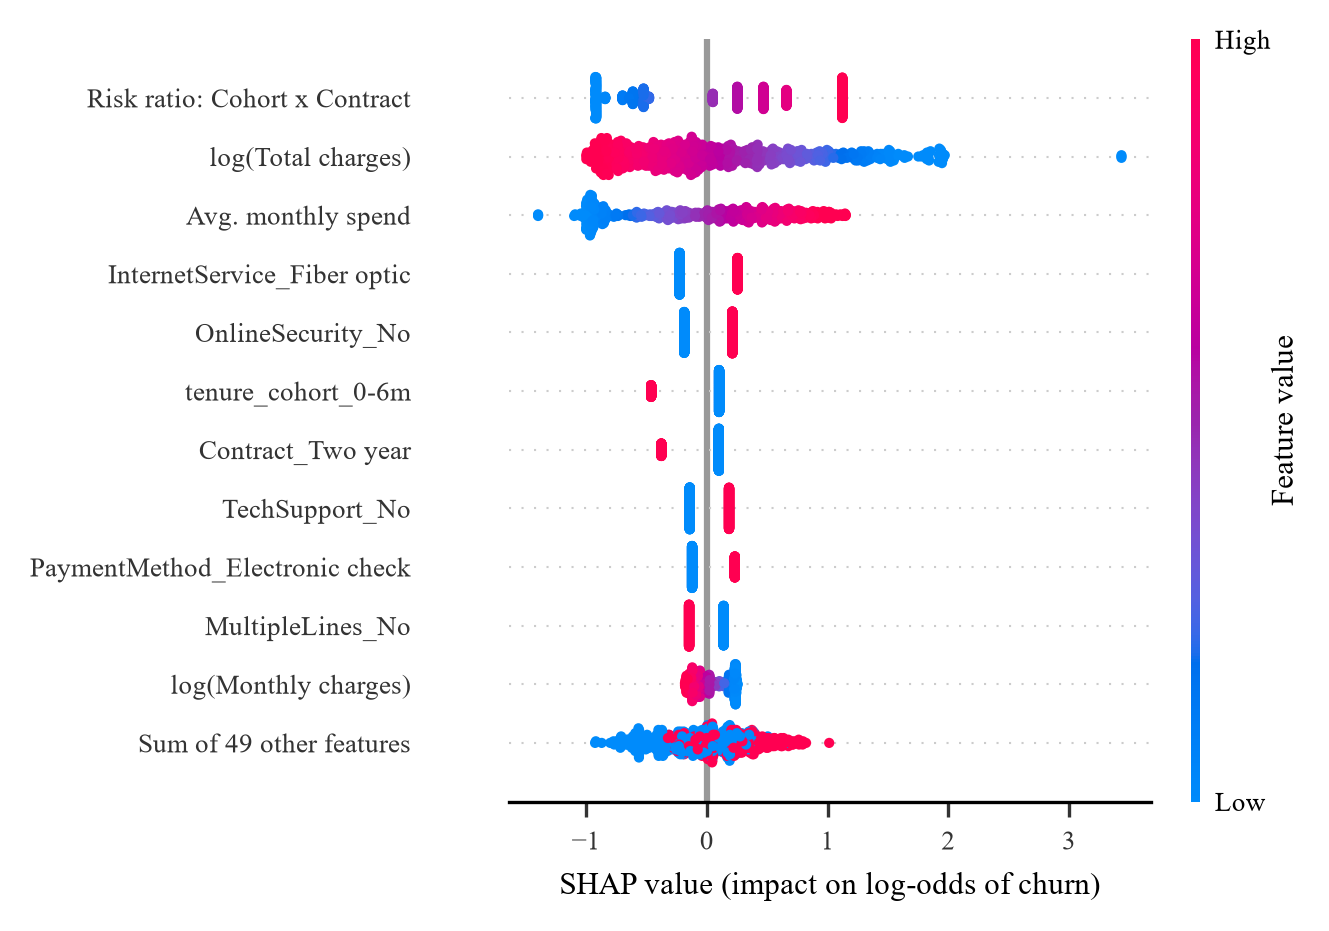
\includegraphics[width=\columnwidth]{shap_summary_light.png}
\caption{Global SHAP summary on 800 holdout customers. Each dot is one customer, and the colour
encodes the feature value.}
\label{fig:shap}
\end{figure}

\begin{table}[t]
\centering
\caption{Global importance: mean $|$SHAP$|$ (log-odds), with one-hot columns aggregated to their
source attribute.}
\label{tab:importance}
\footnotesize
\begin{tabular}{@{}r l l@{}}
\toprule
\textbf{\#} & \textbf{Feature} & \textbf{Mean $|$SHAP$|$}\\
\midrule
\genrows{tab_importance}
\bottomrule
\end{tabular}
\end{table}

\para{Local and counterfactual}\Cref{tab:local} explains one profile: a senior,
single, fiber-optic customer two months into a month-to-month contract, paying \$94.50 by
electronic check, scored at \ExampleP{} churn risk. The dashboard then searches a set of
actionable interventions (contract migration, automatic payment, support and security
bundles, a loyalty discount) and ranks the ones that lower the score. These are
\emph{model-based} what-ifs in the sense of Wachter et al.~\cite{wachter2018counterfactual}: they predict the
outcome for an otherwise identical customer. They are not causal estimates of an offer's uplift,
which still requires controlled experiments.

\begin{table}[t]
\centering
\caption{Local explanation and counterfactual prescriptions for the ``high-risk newcomer''
profile shown in the dashboard (\ExampleP{} predicted churn).}
\label{tab:local}
\footnotesize
\begin{tabularx}{\columnwidth}{@{}L r@{}}
\toprule
\textbf{Top SHAP contributions} & \textbf{log-odds}\\
\midrule
\genrows{tab_local_shap}
\bottomrule
\end{tabularx}

\vspace{6pt}
\begin{tabularx}{\columnwidth}{@{}L r r@{}}
\toprule
\textbf{Counterfactual intervention} & \textbf{New $p$} & \textbf{$\Delta$ pts}\\
\midrule
\genrows{tab_counterfactual}
\bottomrule
\end{tabularx}
\end{table}

% =====================================================================================
\section{Subgroup Audit}
\label{sec:fairness}

\Cref{tab:fairness} compares holdout behaviour across demographic groups at the deployed
threshold. Calibration holds within every group: the mean predicted probability tracks the
observed churn rate. The model behaves almost identically for women and men, consistent with
the $\chi^2$ result in \cref{sec:stats}. Senior citizens, however, have a much higher base rate,
and under a single global threshold they receive roughly double the false-positive rate of other
customers, with lower ranking quality. For a retention offer, a false positive means an
unnecessary benefit, which is acceptable. It would not be acceptable if the score drove any
adverse action. In that case, group-specific thresholds or an equal-opportunity constraint
\cite{hardt2016equality} would be needed. Customers with dependents see lower recall, so
retention outreach may under-serve them.

\begin{table}[t]
\centering
\caption{Subgroup audit on the holdout at $t=\Threshold$. FPR = false-positive rate.}
\label{tab:fairness}
\footnotesize
\setlength{\tabcolsep}{3.6pt}
\begin{tabular}{@{}l r r r r r r@{}}
\toprule
\textbf{Group} & $n$ & \textbf{Churn} & \textbf{Mean $p$} & \textbf{Recall} & \textbf{FPR} & \textbf{AUC}\\
\midrule
\genrows{tab_fairness}
\bottomrule
\end{tabular}
\end{table}

% =====================================================================================
\section{System}
\label{sec:system}

The model ships as a single \code{joblib} artifact with JSON metadata recording the version,
threshold, metrics, holdout fingerprint, library versions and host hardware. A four-page
Streamlit portal (\cref{fig:screens}) provides (i) a real-time risk engine with a calibrated
gauge, local SHAP waterfall and counterfactual cards; (ii) a customer database view over
SQLite or PostgreSQL, with an audit timeline of every logged score; (iii) executive analytics
that recompute the inferential tests live; and (iv) schema-validated batch scoring.
Inputs are validated with Pydantic. Unknown categorical levels are ignored rather than raising
errors, and extra columns such as the label are dropped before scoring, which closes an
inference-time leakage path. A GitHub Actions pipeline runs ruff, mypy and 60
tests, including leakage, determinism and database tests. It also re-scores the committed model
on the fingerprinted holdout and fails if ROC-AUC $<0.82$, PR-AUC $<0.60$, recall $<0.75$ or
Brier $>0.16$.

\begin{figure*}[t]
\centering
\subfloat[Real-time risk engine]{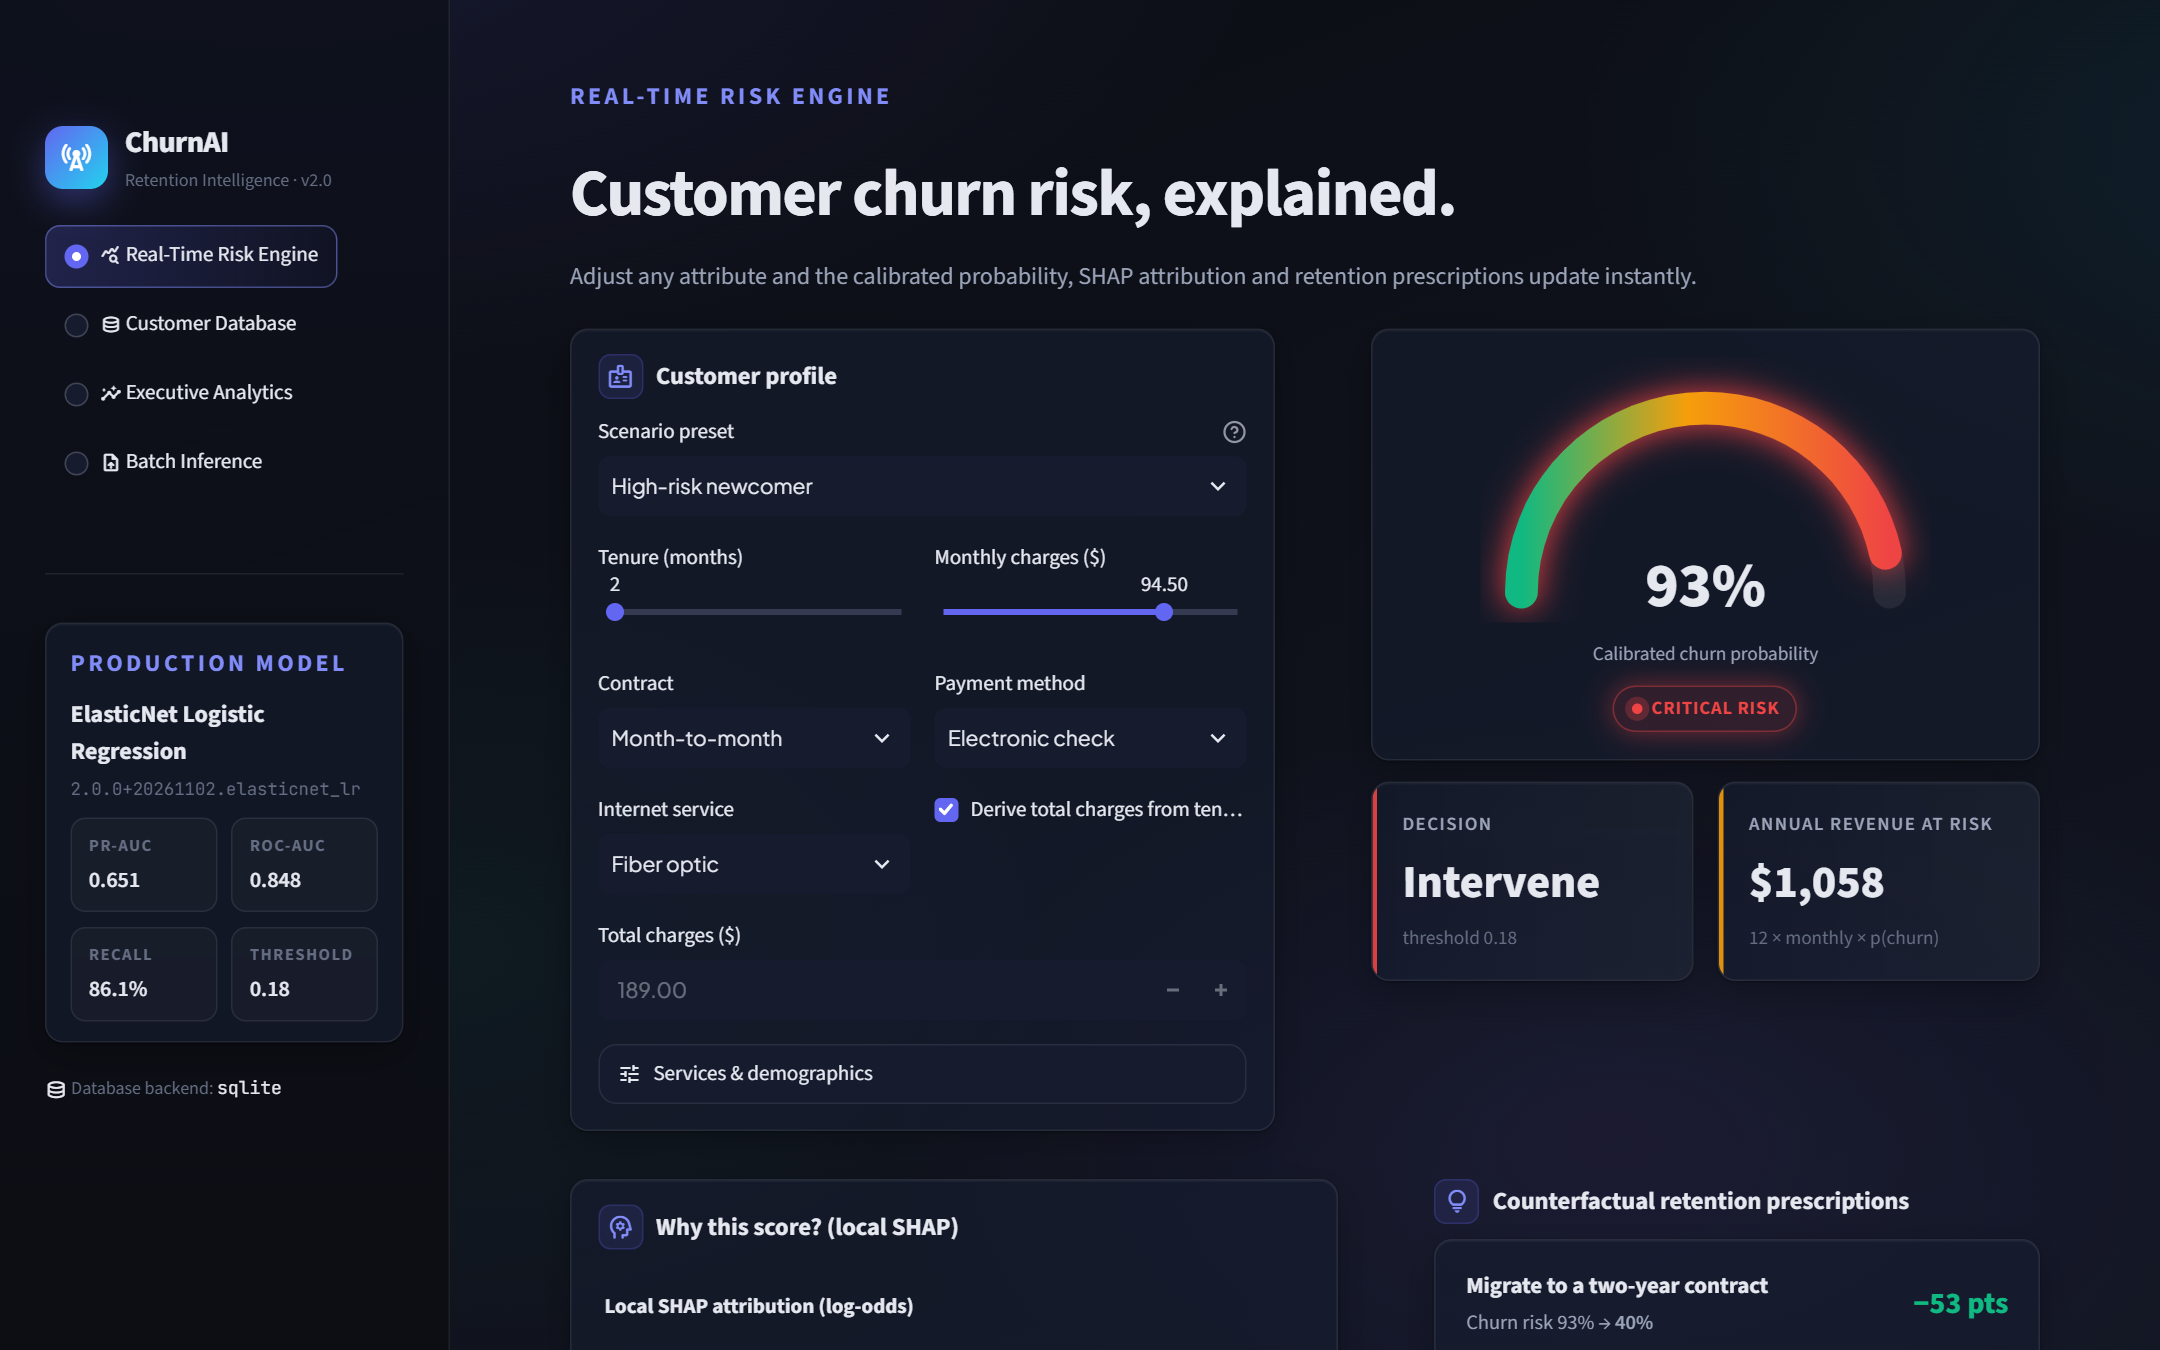
\includegraphics[width=0.485\textwidth]{01_risk_engine.png}}\hfill
\subfloat[Local SHAP and counterfactual prescriptions]{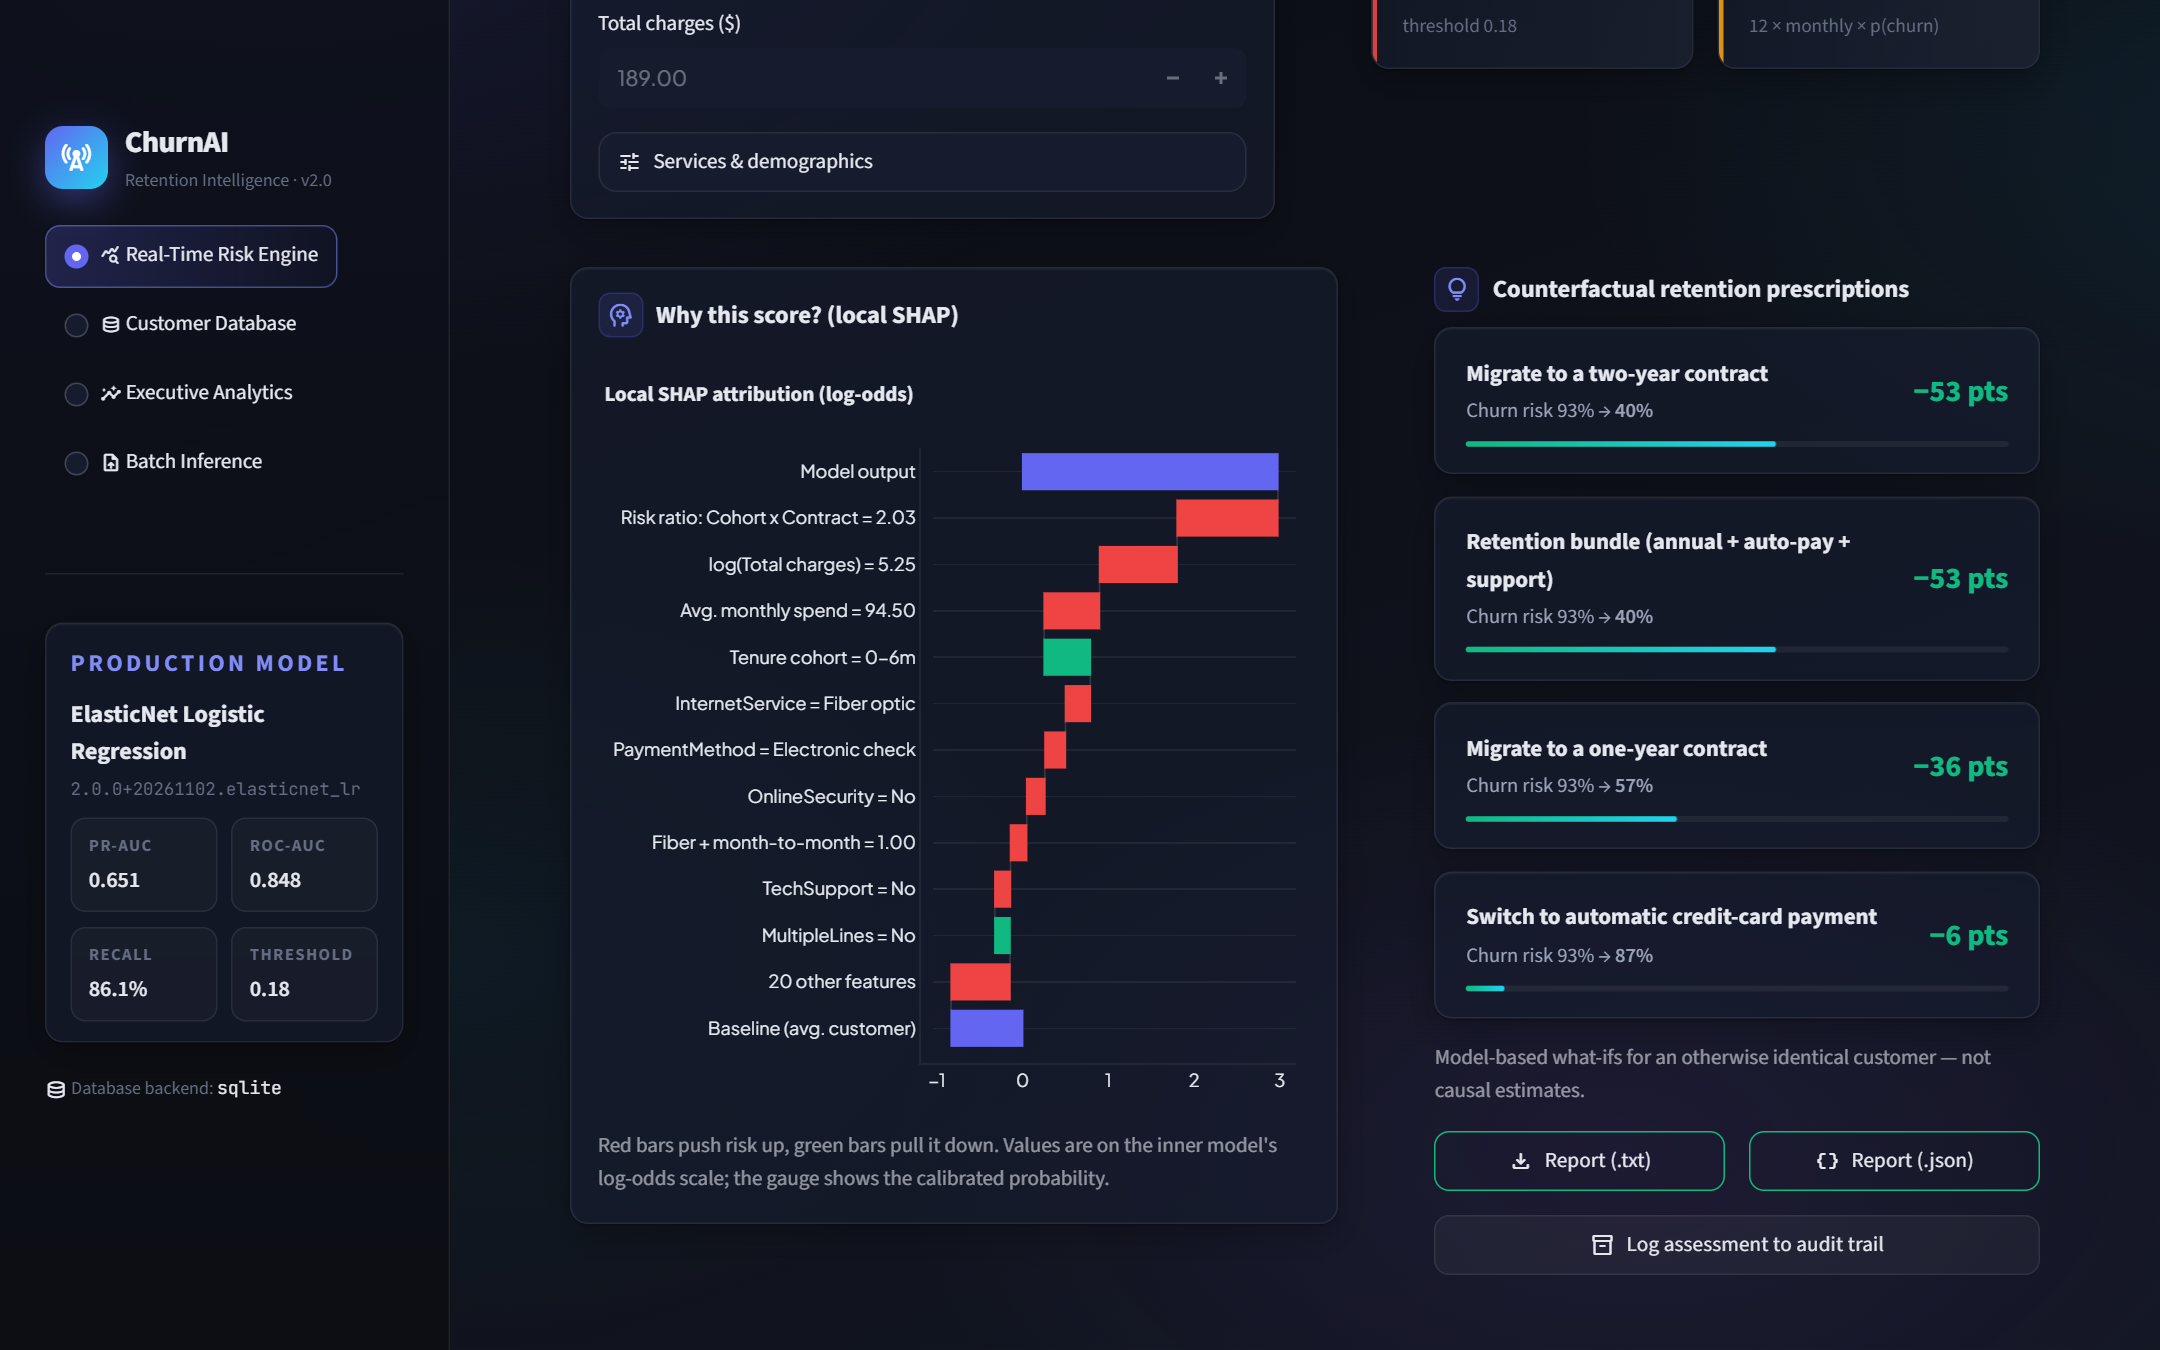
\includegraphics[width=0.485\textwidth]{02_explainability.png}}
\caption{The ChurnAI dashboard. The calibrated probability, risk tier, decision and
revenue at risk update as the profile is edited. Every score can be explained, turned into a
ranked list of retention actions, exported as a report, and logged to the audit trail.}
\label{fig:screens}
\end{figure*}

% =====================================================================================
\section{Limitations and Ethics}
\label{sec:limits}

\para{Data}The dataset is a single snapshot of a fictional provider, with no time
dimension. The model sees customer state, not trajectory (usage decline, support tickets, price
changes), and seasonality and concept drift are not represented. Within long contracts, ranking
quality is weak: at the deployed threshold, none of the two-year-contract churners in the
holdout is flagged. A natural next
step is longitudinal data such as the KKBox churn dataset.
\para{Costs}The 5:1 cost ratio and the \CostUnit{} unit are illustrative. Real offer
costs and customer lifetime values should be substituted, and the threshold re-derived.
\para{Causality}Counterfactual prescriptions are associational. Customers on long
contracts are partly self-selected loyalists, so the predicted risk reduction overstates the
effect of moving a customer onto one. Offers should be validated with A/B tests.
\para{Use}The model is intended to prioritise \emph{beneficial} outreach. It must not
drive adverse actions such as price increases or service downgrades, nor decisions in regulated
domains. Prediction logs contain customer identifiers and should be governed as personal data.

% =====================================================================================
\section{Conclusion}
\label{sec:conclusion}

On the IBM Telco dataset, careful protocol matters more than model complexity. A regularised
logistic regression, evaluated without leakage, calibrated, and operated at a cost-derived
threshold, matches or beats gradient boosting and stacking. It cuts expected loss by
\LossSavingNone{} relative to inaction, while remaining fast, exactly explainable and easy to
audit. Most of the practical value comes from steps that are often skipped: confirming drivers
statistically, calibrating, choosing the threshold out of sample, explaining individual
decisions and auditing subgroups. ChurnAI packages these steps into a reproducible,
tested and documented system.

% =====================================================================================
\section*{Appendix: Reproducibility}

Every number, table and chart in this report is generated from the committed model and data by
\code{scripts/build\_paper.py}. All experiments ran locally on a single laptop CPU, with no GPU
or cloud compute (\cref{tab:env}). The full tournament, including the 30-iteration tuning
search, takes about ten minutes.

\begin{table}[h]
\centering
\caption{Computing environment.}
\label{tab:env}
\footnotesize
\begin{tabularx}{\columnwidth}{@{}l L@{}}
\toprule
Machine & ASUS Zenbook 14 (UX3405CA), laptop\\
CPU & \HWcpu{} (\HWthreads{} threads)\\
Memory & \HWram{}\,GB\\
OS & \HWos{}\\
Python & \PyVersion{}, dependencies pinned with \code{uv.lock}\\
Libraries & scikit-learn \SklearnVersion{}, XGBoost \XGBVersion{}, LightGBM \LGBMVersion{}, CatBoost \CatBoostVersion{}, SHAP \ShapVersion{}, pandas \PandasVersion{}, NumPy \NumpyVersion{}\\
Seed & 42 (split, CV, learners)\\
\bottomrule
\end{tabularx}
\end{table}

\noindent\textit{Commands.}\par\smallskip
{\footnotesize
\begin{tabular}{@{}l@{}}
\code{uv sync --all-extras}\\
\code{uv run python -m src.models.train --tune-iter 30}\\
\code{uv run python -m src.models.evaluate --validate-thresholds}\\
\code{uv run python scripts/build\_paper.py}\\
\code{uv run streamlit run src/ui/app.py}\\
\end{tabular}}

\bibliographystyle{IEEEtran}
\bibliography{references}

\end{document}
